\documentclass[11pt, openright, a4paper, brazil, openany, oneside]{abntex2}
\usepackage{lmodern}
\usepackage{verbatim}
\usepackage[T1]{fontenc}	
\usepackage[utf8]{inputenc}
\usepackage{times}	
\usepackage{indentfirst}	
\usepackage{color}			
\usepackage{graphicx}		
\usepackage{microtype} 		
\usepackage{multicol}
\usepackage{multirow}
\usepackage{lipsum}				
\usepackage[brazilian,hyperpageref]{backref}	 
\usepackage[alf]{abntex2cite}
\renewcommand{\backrefpagesname}{Citado na(s) página(s):~}
\renewcommand{\backref}{}
\renewcommand*{\backrefalt}[4]{
	\ifcase #1 %
		Nenhuma citação no texto.%
	\or
		Citado na página #2.%
	\else
		Citado #1 vezes nas páginas #2.%
	\fi}%
\titulo{Cálculo Numérico}
\autor{Sérgio Luís Soares Almeida \\ Matrícula 18/0006410}
\local{Brasília}
\data{2018, 02 de Outubro}
\instituicao{%
  Universidade de Brasília -- UnB
  \par
  Departamento de Matemática
  \par
 PROFMAT
  \par
  Professor José Eduardo Castilho}
\tipotrabalho{Relatório}

\definecolor{black}{RGB}{0.0,0.0,0.0}


\makeatletter
\hypersetup{pdftitle={\@title}, pdfauthor={\@author}, pdfsubject={\imprimirpreambulo}, pdfcreator={LaTeX with abnTeX2}, pdfkeywords={abnt}{latex}{abntex}{abntex2}{relatório técnico}, colorlinks=true, linkcolor=black, citecolor=black, filecolor=black, urlcolor=black, bookmarksdepth=4}
\makeatother

\setlength{\parindent}{1.3cm}


\setlength{\parskip}{0.2cm}  


\makeindex

\begin{document}


\selectlanguage{brazil}


\frenchspacing 


\imprimircapa

\imprimirfolhaderosto*

\ABNTEXchapterfont

\pdfbookmark[0]{\contentsname}{toc}
\tableofcontents*
\cleardoublepage
\textual

\chapter*[Introdução]{Introdução}
\addcontentsline{toc}{chapter}{Introdução}


A disciplina de Cálculo Numérico do curso de Mestrado Profissional de Matemática - PROFMAT incentiva a usar os recursos computacionais para resolver alguns problemas matemáticos e, para isso, será usado o programa \textit{Octave} para desenvolver alguns projetos. O programa \textit{Octave} foi desenvolvido através da licença \textbf{GNU} e pode ser baixado facilmente através do site https://www.gnu.org para diversas plataformas.

Neste segundo relatório faremos 3 projetos envolvendo o Método dos Mínimos Quadrados, a Regra de Simpson para integrais e o Método de Euler para Problemas de Valores Iniciais.




\chapter{Método dos Mínimos Quadrados}

Neste projeto desenvolvemos um programa no \textit{Octave} para implementar um caso de ajuste por um polinômio de grau $n$ pelo Método dos Mínimos Quadrados: 

\begin{verbatim}

function [funcao,coeficientes]=MMQ(x,f,g) #x é a matriz com valores de x, f a matriz f(x) e g o grau
A=zeros(g+1);
b=zeros(g+1,1);
faux=zeros(g+1,length(x));
for i=1:g+1
  for j=1:length(x)
    faux(i,j)=x(1,j)^(i-1);
  endfor
endfor
for i=1:g+1
  for j=1:g+1
    for k=1:length(x)
      A(i,j)=A(i,j)+faux(i,k)*faux(j,k);
    endfor
  endfor
  for k=1:length(x)
     b(i,1)=b(i,1)+f(1,k)*faux(i,k);
  endfor
endfor
coeficientes=EGauss(A,b);
funcao=zeros(size(x));
for i=0:g
     funcao=funcao+(x.^i)*coeficientes(i+1);
   endfor
  plot(x,f,'*r',"linewidth",2,x,funcao,'-b',"linewidth",2)
  D=sum((f-funcao).^2)
endfunction

\end{verbatim}

Esse programa foi salvo com o nome de "MMQ.m". Dessa forma, o \textit{Octave} poderá encontrar os valores dos coeficientes de um polinômio e fazer um gráfico que se aproxima dos valores coletados digitando os dados de $x$, de $f(x)$ em cada um desses pontos e do grau do polinômio desejado.

Inserimos nesse programa os dados de x e f(x) conforme as tabelas abaixo:

\begin{center}
\begin{tabular}{c||c|c|c|c|c|c}

x & 0.1 & 0.2 & 0.3 & 0.4 & 0.5 & 0.6 \\ \hline\hline
f(x)&0.101&0.209&0.335&0.489&0.687&0.945\\ \hline\hline\hline

\end{tabular}

\begin{tabular}{c||c|c|c|c|c|c}

x & 0.7 & 0.8 & 0.9 & 1.0 & 1.1 & 1.2 \\ \hline\hline
f(x) &1.283&1.721&2.285&3.000&3.895&5.001
\end{tabular}
\end{center}

Podemos ver o resultado através da figura \ref{octave1} e o gráfico através da figura ???

\begin{figure}[h]

    \center

    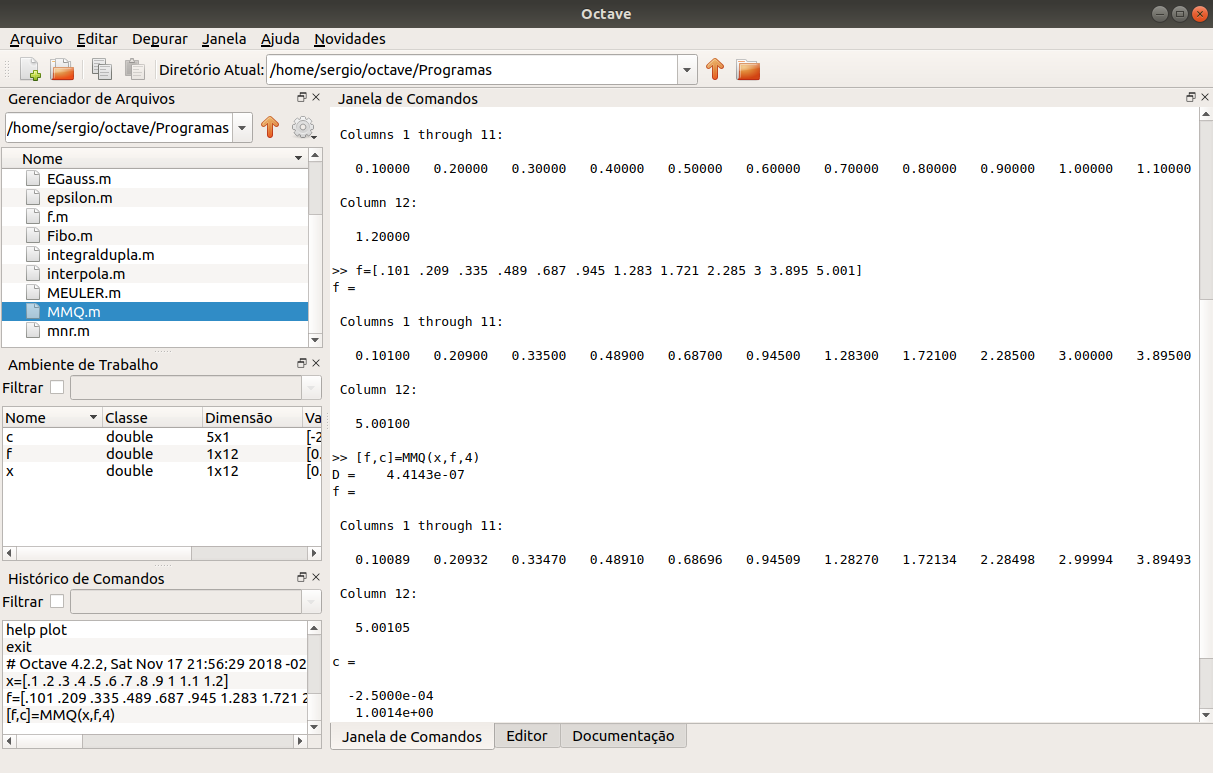
\includegraphics[width=12cm]{octave1.png}
    \caption{Precisões da Máquina e do \textit{Octave} \label{octave1}}
    
\end{figure}


\section{Resultados}

Podemos observar pelos resultados e pelo gráfico que, neste caso, a aproximação é excelente, o que nos mostra que esse é um método muito eficiente.


\chapter{Regra de Simpson}



Encontrar essa raiz é equivalente a encontrar o zero da função $ f(x) = x^p - a $.

\section{Encontrando um intervalo}

A primeira questão consiste em encontrar um intervalo que depende de $a$ e que contenha a raiz. Como queremos uma raiz positiva, podemos separar em duas situações: $a<1$ e $a>1$ 

\begin{itemize}
\item Se $a<1$, multiplicando os dois lados por $a$, $p$ vezes,  temos que:

\begin{center}


$a^2<a$  \\ $a^3<a^2<a$ \\ $ \vdots $ \\ $a^p< \cdots < a^3 < a^2 < a$

\end{center}

Então: 
\begin{center}

$ a^p<a<1 $

$ \sqrt[p]{a^p}<\sqrt[p]{a}<\sqrt[p]{1} $

$ a<\sqrt[p]{a}<1 $


\end{center}

Assim podemos usar o intervalo $[a,1]$.

\item Se $a>1$, como queremos usar um intervalo que depende de $a$, e como queremos apenas uma raiz positiva, ela será menor que $a$, logo podemos usar o intervalo $[1,a]$.


\end{itemize}

\section{Critérios de Convergência}

Nesta seção verificaremos se a função de iteração $ \phi (x) = \frac{a}{x^{p-1}} $ satisfaz os critérios de convergência do Método Iterativo Linear.

\begin{enumerate}

\item Levando em consideração os intervalos citados na seção anterior para os valores de $a$, a função $ \phi (x) = \frac{a}{x^{p-1}} $ é contínua. Devemos então calcular a sua derivada:
\begin{center}
$ \phi (x) = \frac{a}{x^{p-1}} = a \cdot x^{1-p} $ \\ $ \phi ' (x) = a \cdot (1-p) \cdot x^{-p}$ \\  $ \phi ' (x) = \frac {a \cdot (1-p)}{x^p}$

\end{center}

Assim, $ \phi '(x) $ também é contínua nos intervalos considerados.

\item Aqui temos 2 casos:

\begin{itemize}

\item Se $a<1$ escolhemos anteriormente o intervalo $[a,1]$. Seja $x \in [a,1]$, então $x^p\le 1$, mas $\frac{1}{x^p}\geq1$, então, como $p\geq2$ , podemos tomar, por exemplo, $x=a$, e assim:

\begin{center}

$ \left| \phi ' (x)\right| = \left| \frac {a \cdot (1-p)}{x^p} \right|= \left| \frac {a \cdot (1-p)}{a^p} \right| = \left|\frac{1-p}{a^{p-1}} \right| \geq1$

\end{center}

Desta forma, no intervalo $[a,1]$ não podemos afirmar a sua convergência.

\item Se $a>1$, como escolhemos o intervalo $[1,a]$, podemos escolher $x=1$, e assim temos:

\begin{center}

 $ \left| \phi ' (x)\right| = \left| \frac {a \cdot (1-p)}{x^p} \right| = \left| a \cdot (1-p)\right|$

\end{center}

E assim, como $p\geq2$ e $a\geq1$, temos que $|\phi(x)'|$ será maior que 1 e novamente não podemos afirmar a sua convergência.

\end{itemize}

\end{enumerate}

\section{M.N.R para raízes}

Vamos usar o Método de Newton-Raphson para gerar um processo iterativo que encontra a raiz p-ésima positiva de um número $a$ também positivo. Para isso, temos que:

\begin{center}

$ x_{n+1} = x_k - \frac{f(x_k)}{f'(x_k)}$ \\ $ x_{n+1} = x_k - \frac{x^p - a }{p \cdot {x_k}^{p-1}}$ \\ $ x_{n+1} = x_k - \left[ \frac{x^p}{p \cdot {x_k}^{p-1}} - \frac{a}{p \cdot {x_k}^{p-1}} \right]$ \\ $ x_{n+1} = x_k -  \frac{x^p}{p \cdot {x_k}^{p-1}} + \frac{a}{p \cdot {x_k}^{p-1}} $ \\ $ x_{n+1} = \frac {p \cdot x_k -  {x_k}}{p} + \frac{a}{p \cdot {x_k}^{p-1}} $ \\ $ x_{n+1} = \frac {1}{p} \left[( p-1)x_k + \frac{a}{{x_k}^{p-1}} \right] $

\end{center}

\section{Implementando o Programa de Iteração}

Para calcularmos a raiz p-ésima positiva do número $a$ usaremos o seguinte programa:

\begin{verbatim}
function y=newrap(a,p,Ep)
  x0=a;
  x1=(1/p)*((p-1)*a+(a/(a^(p-1))));
  while (abs(x1-x0)>Ep)
    x0=x1;
    x1=(1/p)*((p-1)*x0+(a/(x0^(p-1))));
  endwhile
  y=x1;
 endfunction
\end{verbatim}

Onde os valores $a$, $p$ e $Ep$ são respectivamente o radicando, o índice e a precisão da raiz. 

O programa deve ser salvo com o mesmo nome da função, neste caso foi \textbf{newrap} (NEWton-RAPhson) e para calcular por exemplo a raiz 5\textsuperscript{\d a} de 8 com uma precisão de $10^{-10}$, na janela de comandos do \textit{Octave}, escrevemos o comando \textbf{y=newrap(8,5,10}\verb|^|\textbf{(-10))}, como podemos ver na figura \ref{octave2}.


\begin{figure}[h]

    \center

    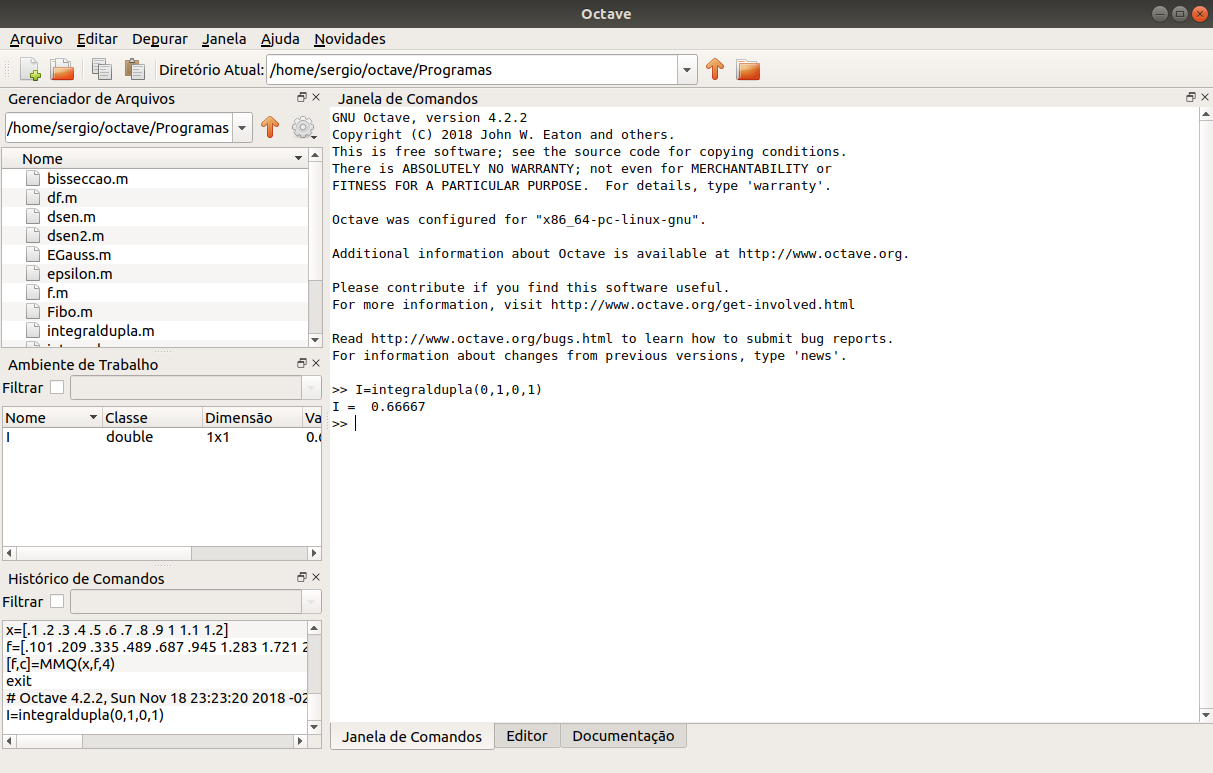
\includegraphics[width=12cm]{octave2.png}
    \caption{retirando raízes p-ésimas \label{octave2}}
    
\end{figure}

\section{Resultados}

Podemos observar que pelo Método Newton-Raphson a forma de determinar uma raiz p-ésima através da iteração $ x_{n+1} = \frac {1}{p} \left[( p-1)x_k + \frac{a}{{x_k}^{p-1}} \right] $ é muito eficaz computacionalmente e que, mesmo que $ \phi ' (x) = \frac {a \cdot (1-p)}{x^p}$ seja maior que 1, ele converge e com uma ótima precisão.

\newpage

\chapter{Projeto 3 - Sistemas Lineares}

Neste projeto vamos fazer um programa para resolver o sistema:

\begin{center}

$\left[ \begin{array}{ccccccccccccccccc}

8x_1 & + & x_2 & + & x_3 & + & x_4 & + & x_5 & + & x_6 & + & x_7 & + & x_8 & = & 15 \\ x_1 & + & 8x_2 & + & x_3 & + & x_4 & + & x_5 & + & x_6 & + & x_7 & + & x_8 & = & 15 \\ x_1 & + & x_2 & + & 8x_3 & + & x_4 & + & x_5 & + & x_6 & + & x_7 & + & x_8 & = & 15 \\ x_1 & + & x_2 & + & x_3 & + & 8x_4 & + & x_5 & + & x_6 & + & x_7 & + & x_8 & = & 15 \\ x_1 & + & x_2 & + & x_3 & + & x_4 & + & 8x_5 & + & x_6 & + & x_7 & + & x_8 & = & 15 \\ x_1 & + & x_2 & + & x_3 & + & x_4 & + & x_5 & + & 8x_6 & + & x_7 & + & x_8 & = & 15 \\ x_1 & + & x_2 & + & x_3 & + & x_4 & + & x_5 & + & x_6 & + & 8x_7 & + & x_8 & = & 15 \\ x_1 & + & x_2 & + & x_3 & + & x_4 & + & x_5 & + & x_6 & + & x_7 & + & 8x_8 & = & 15

\end{array} \right]$


\end{center}

O programa desenvolvido foi:
\begin{verbatim}

function y=GaussSeidel(a,b,Ep)
  x0=b*0;
  n=length(a);
  m=linspace(1,1,length(b))';
  while (norm(m)>Ep)
    for t=1:n
      p=0;
      for i=1:t-1
        p=p+a(t,i)*x0(i);
      endfor
      for i=t+1:n
        p=p+a(t,i)*x0(i);
      endfor
      x(t)=(b(t)-p)\a(t,t);
    endfor
    m=x-x0;
    x0=x;
  endwhile
  y=x;
 endfunction
 
\end{verbatim}

O programa foi salvo com o nome de \textbf{GaussSeidel.m} e para usá-lo digitamos \textbf{y = GaussSeidel(a,b,ep)} onde \textbf{a} é a matriz dos coeficientes, \textbf{b} é a matriz das constantes e \textbf{ep} é a precisão da norma.

O sistema dado foi resolvido declarando cada variável antes e o resultado podemos ver na figura \ref{octave3}.

\begin{figure}[h]

    \center

    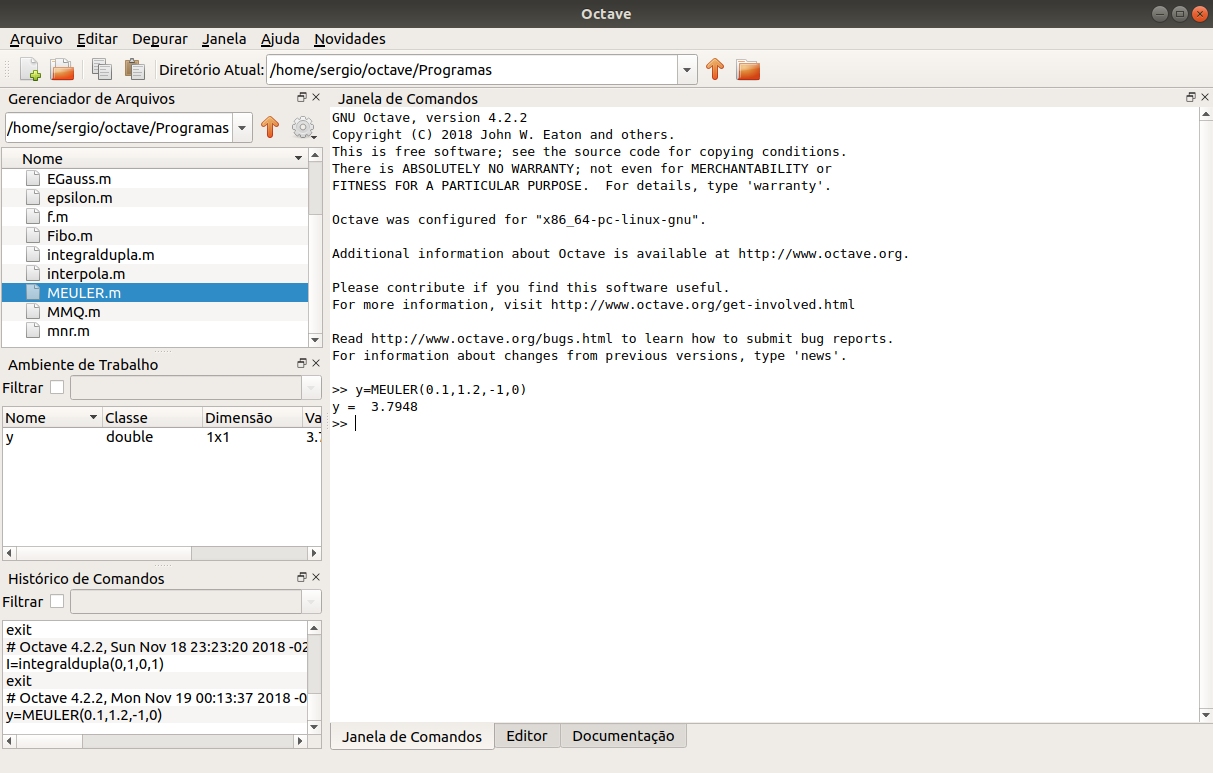
\includegraphics[width=12cm]{octave3.png}
    \caption{solução do sistema linear \label{octave3}}
    
\end{figure}


\section{Resultado}

Podemos perceber que o resultado é bem próximo de 1 para todos as variáveis, isto é, temos uma boa precisão com este programa.


\newpage

\end{document}
